\section{Results}
\label{sec:Results}

\subsection{Dataset scaling type's effects}
Many machine learning algorithms perform better when numerical input variables are scaled to a standard range.

Fizemos três diferentes avaliações. Tendo como referência um lag de 5, avaliamos a influência causada pelos diferentes tipos de transformações utilizadas para escalar os dados.


\begin{center}
\begin{tabular}{ |c|c|c|c|c|c| } 
\hline
Type & Validation RMSE & Validation MAE & Test RMSE & Test MAE \\
\hline
% \multirow{3}{4em}{Multiple row} & cell2 & cell3 \\ 
MinMaxScaler & 0.03555 & 0.01364 & 0.0065 & 0.00459 \\ 
RobustScaler & 0.09398 & 0.03578 & 0.01789 & 0.01354 \\
StandardScaler & 0.13415 & 0.04909 & 0.03254 & 0.02179 \\
\hline
\end{tabular}
\label{tab:scaling_type}
\end{center}

Como podemos observar na tabela \ref{tab:scaling_type}, fazendo a transformação por meio da função de minmax, temos os melhores resultados nos dados de validação e também nos dados de teste.

\subsection{Impact of the quantity of data lags}

\begin{figure}[h!]
    \centering
    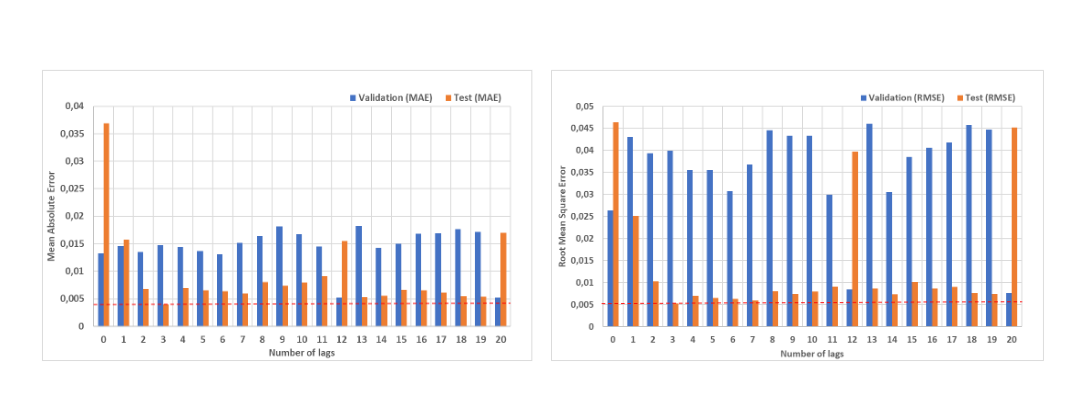
\includegraphics[width=1.0\textwidth]{images/Lag_metrics.png}
    \caption{Lag metrics}
    \label{fig:lag_metrics}
\end{figure}

\begin{figure}[h!]
    \centering
    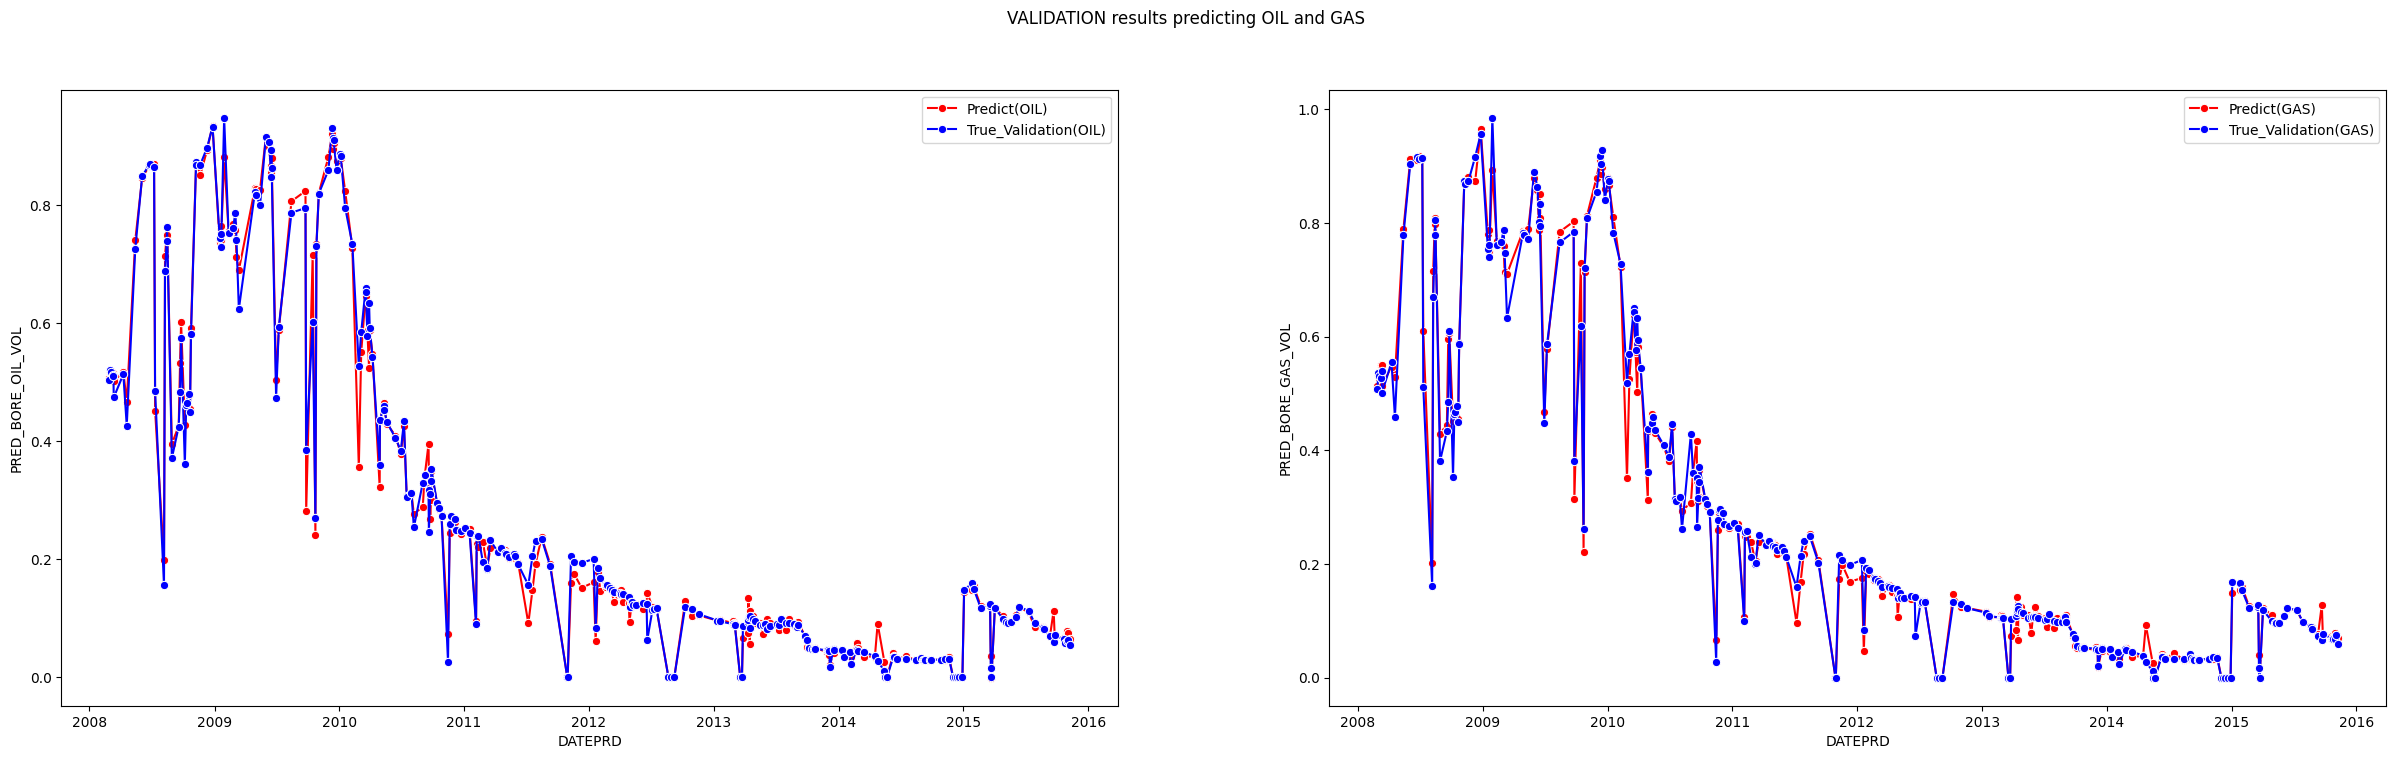
\includegraphics[width=1.0\textwidth]{images/Validation_lag_0.png}
    \caption{Validation 0}
    \label{fig:Val_0}
\end{figure}

\begin{figure}[h!]
    \centering
    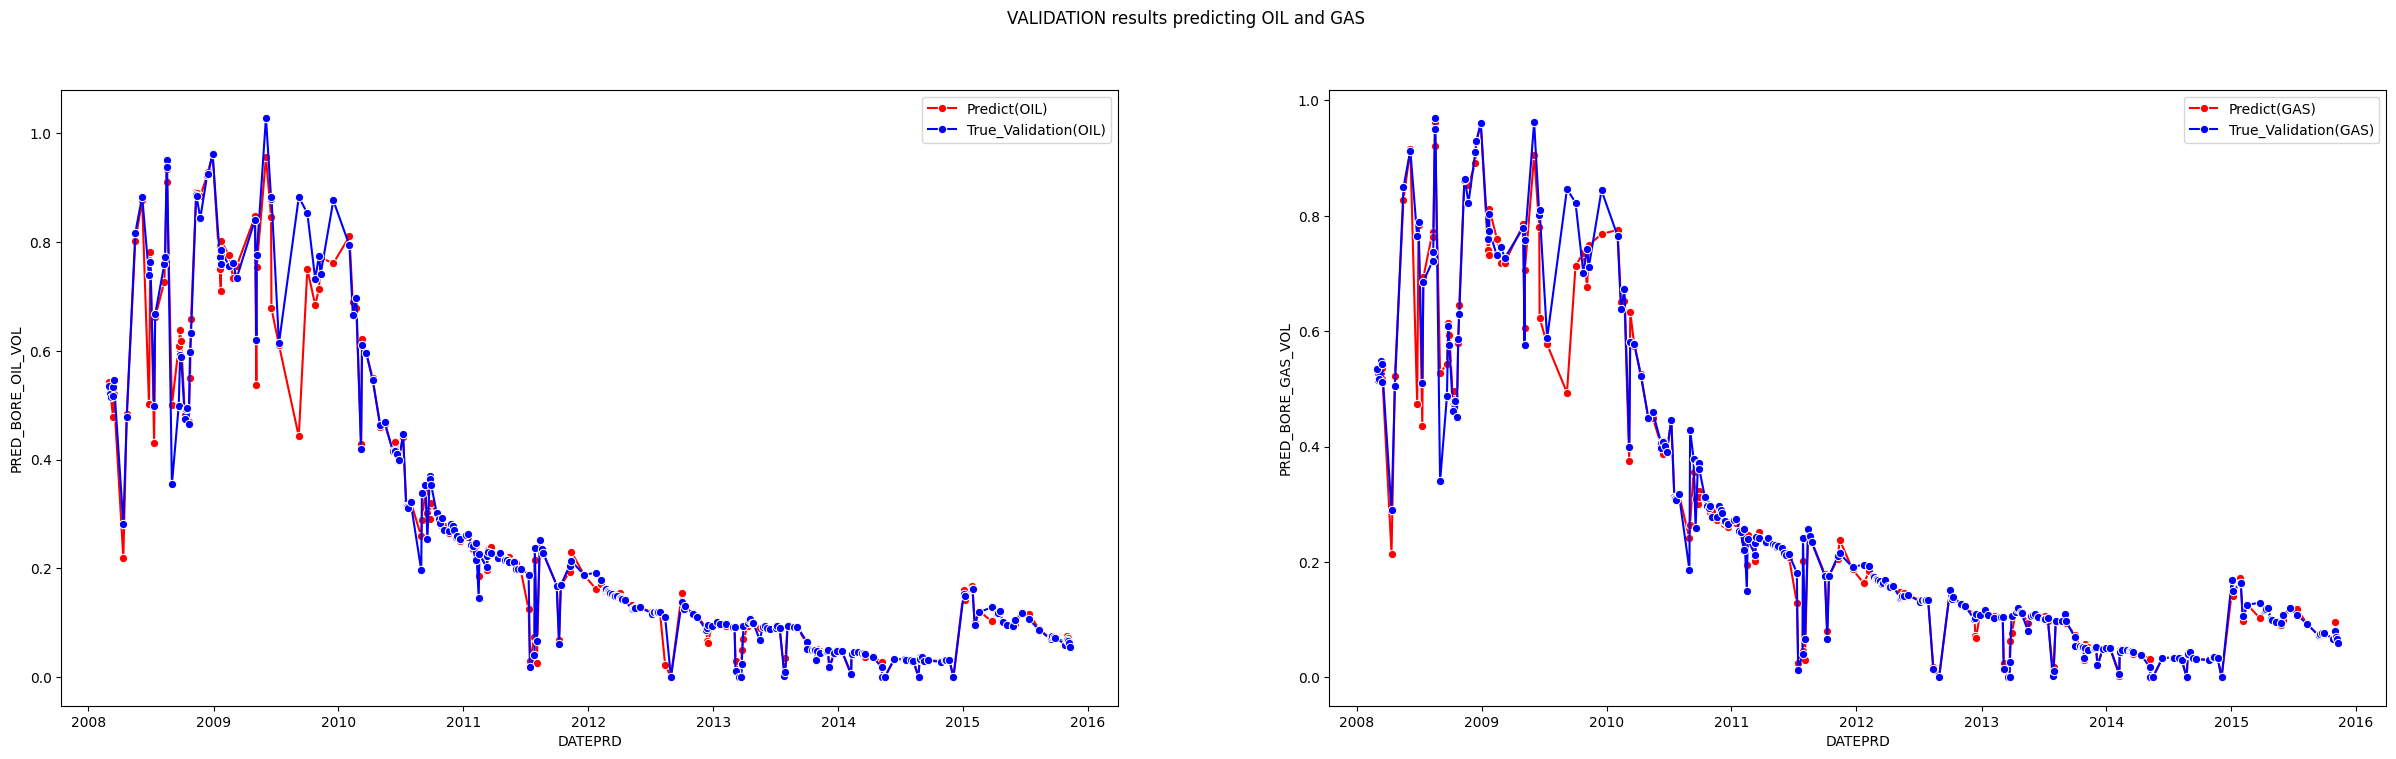
\includegraphics[width=1.0\textwidth]{images/Validation_lag_3.png}
    \caption{Validation 3}
    \label{fig:Val_3}
\end{figure}

\begin{figure}[h!]
    \centering
    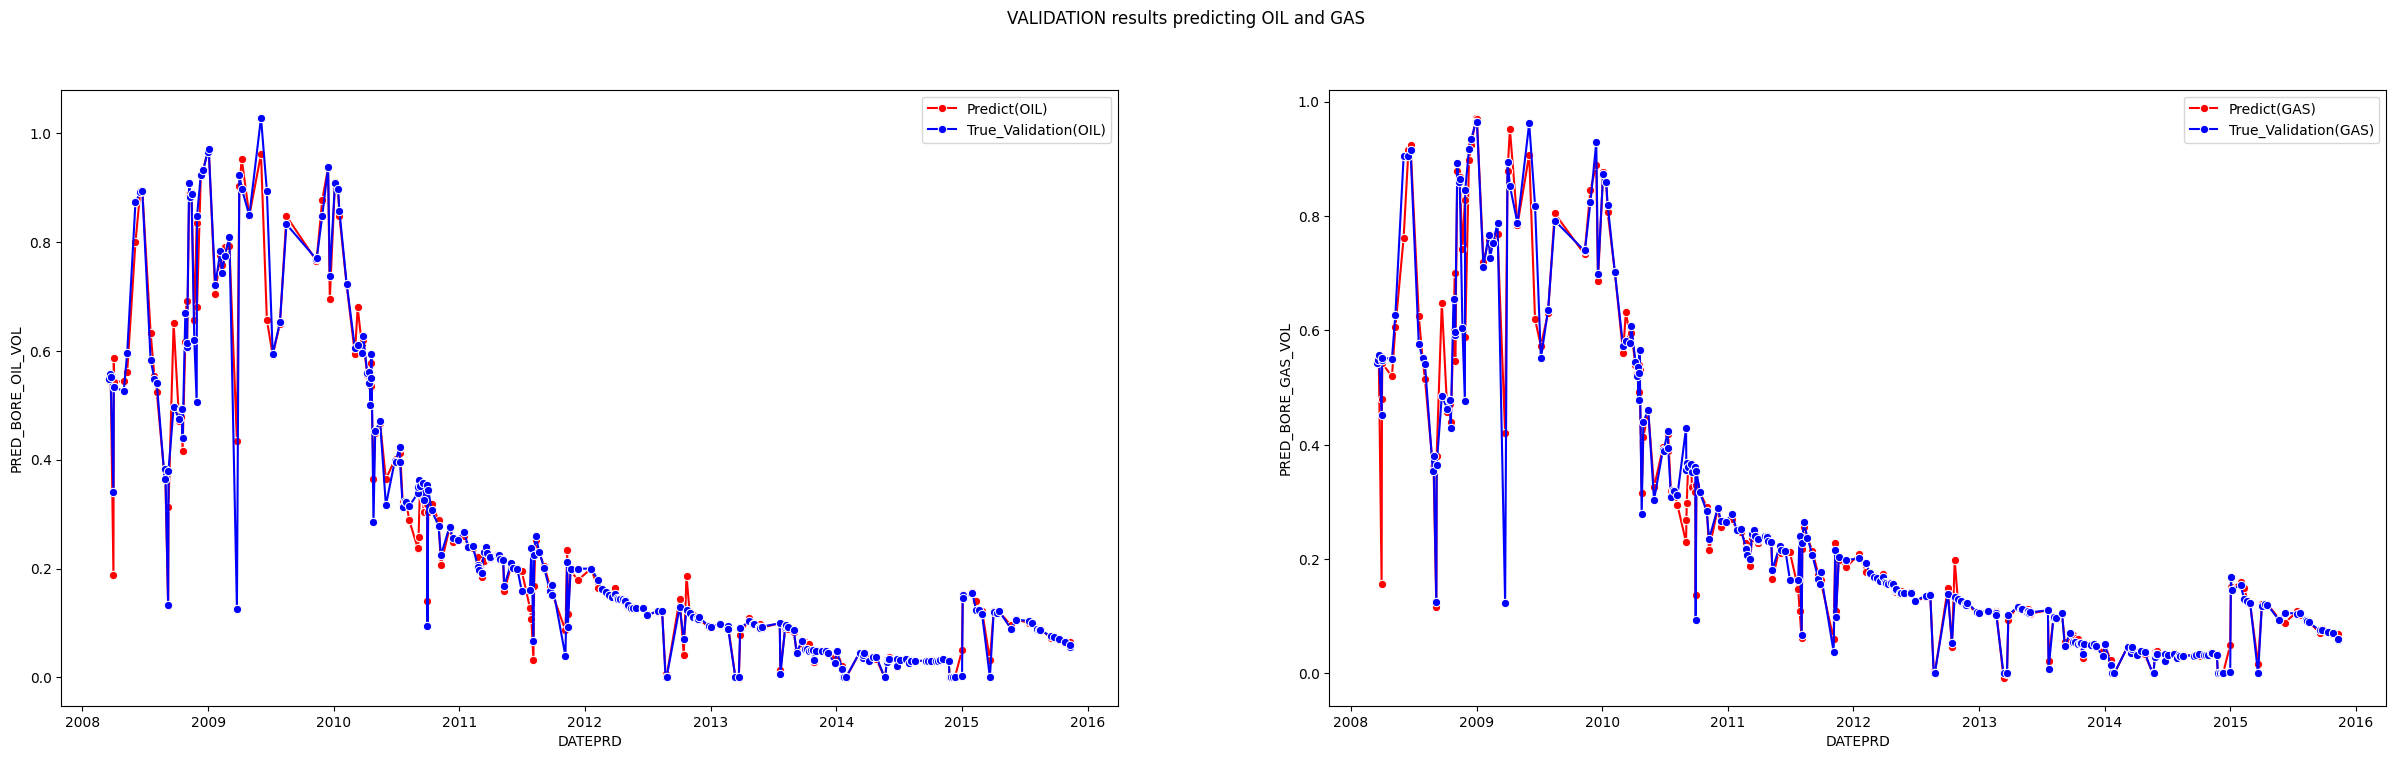
\includegraphics[width=1.0\textwidth]{images/Validation_lag_20.png}
    \caption{Validation 20}
    \label{fig:Val_20}
\end{figure}


\begin{figure}[h!]
    \centering
    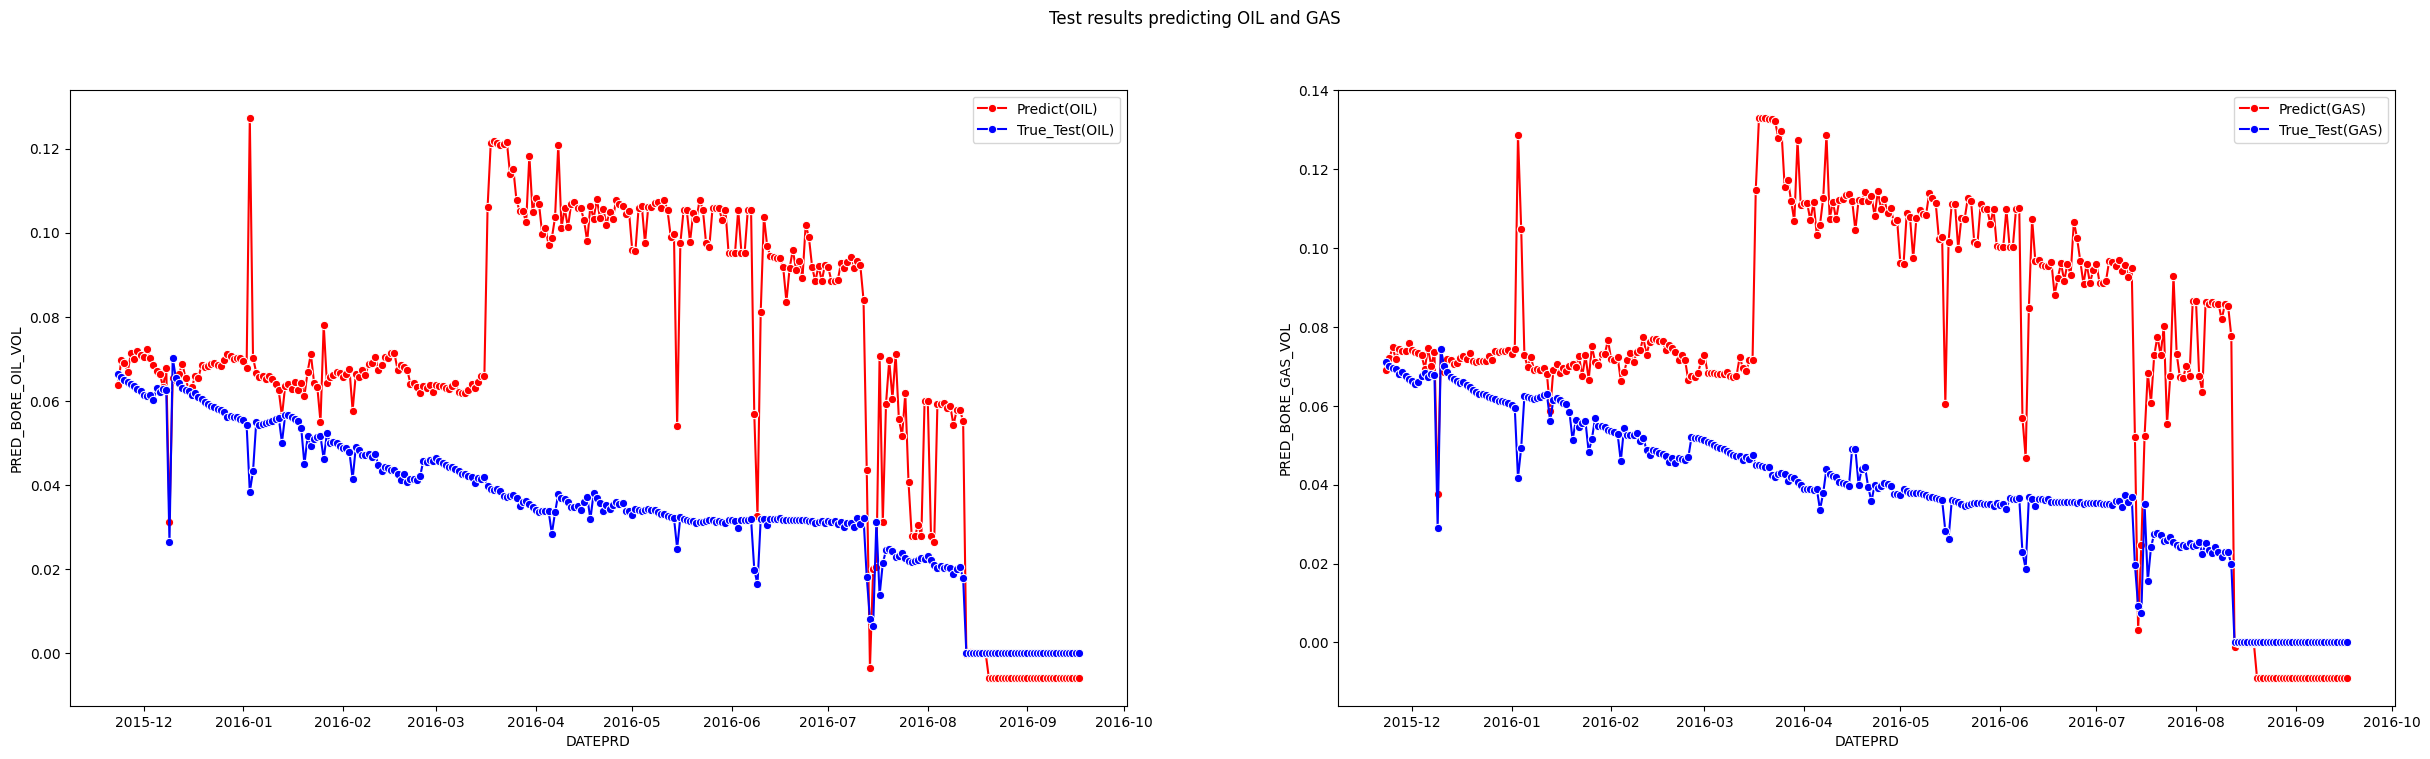
\includegraphics[width=1.0\textwidth]{images/Teste_lag_0.png}
    \caption{Test 0}
    \label{fig:Test_0}
\end{figure}

\begin{figure}[h!]
    \centering
    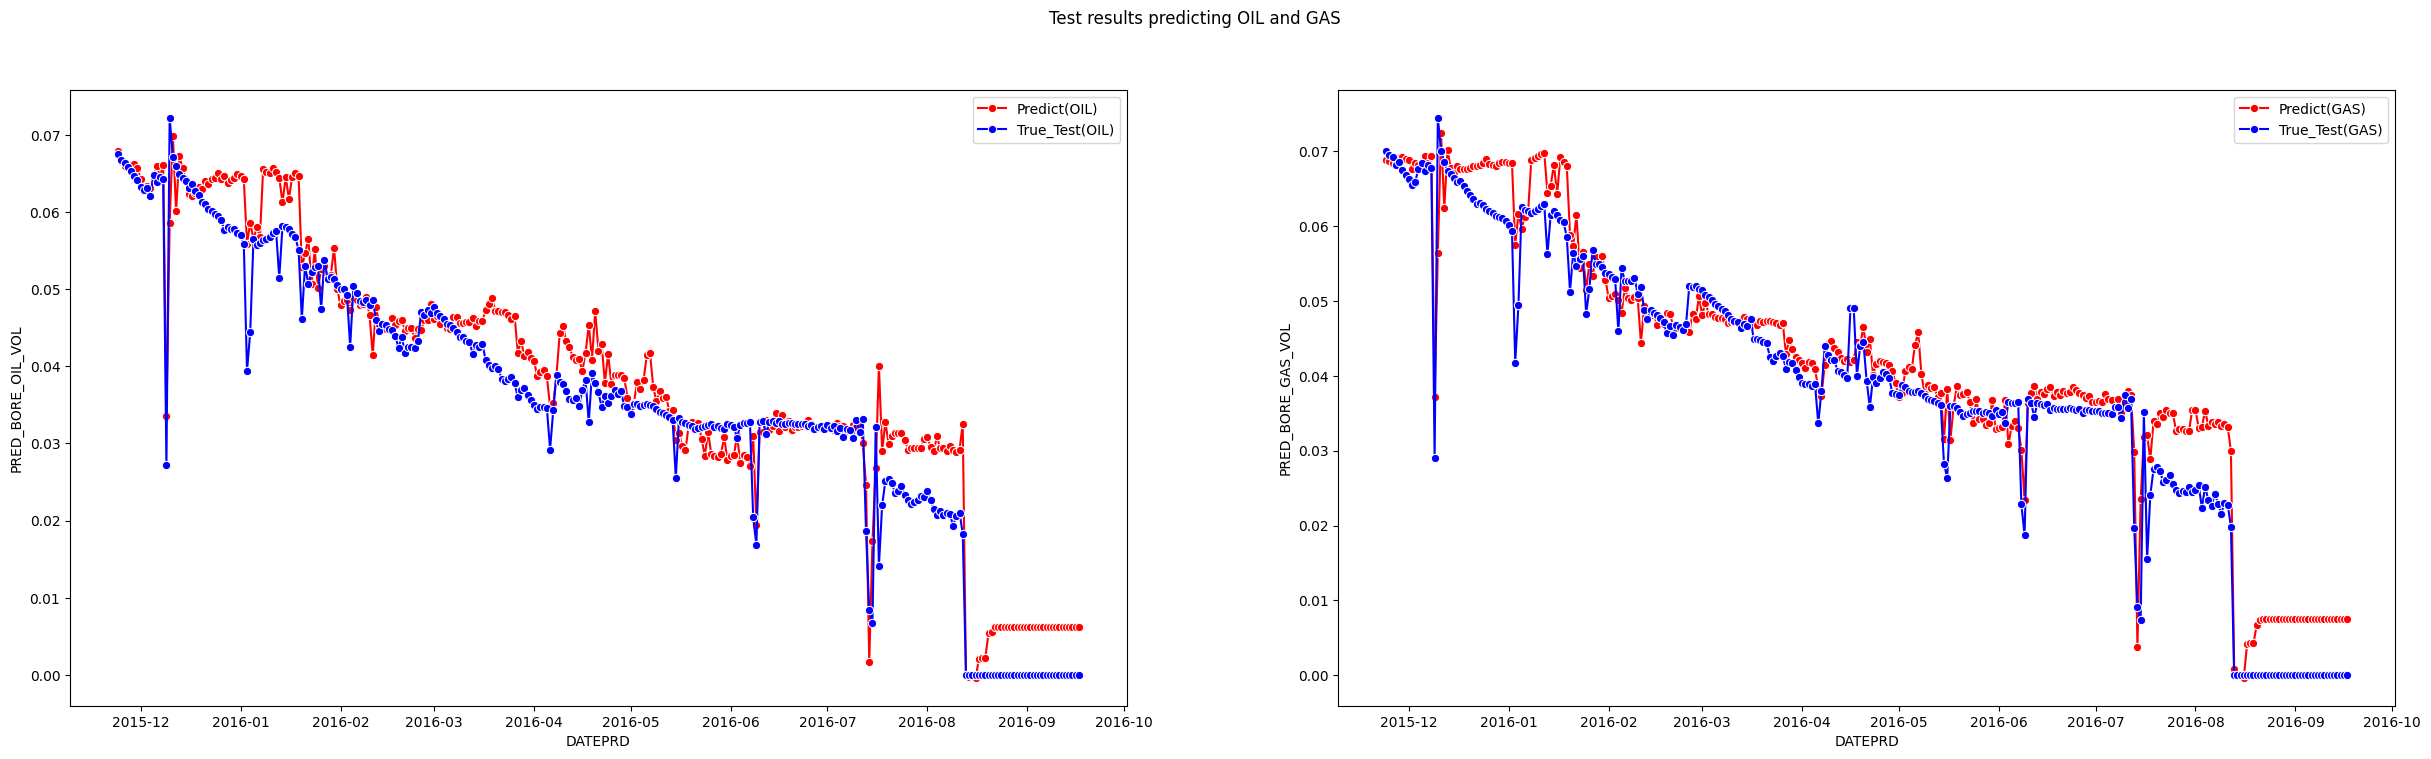
\includegraphics[width=1.0\textwidth]{images/Teste_lag_3.png}
    \caption{Test 3}
    \label{fig:Test_3}
\end{figure}

\begin{figure}[h!]
    \centering
    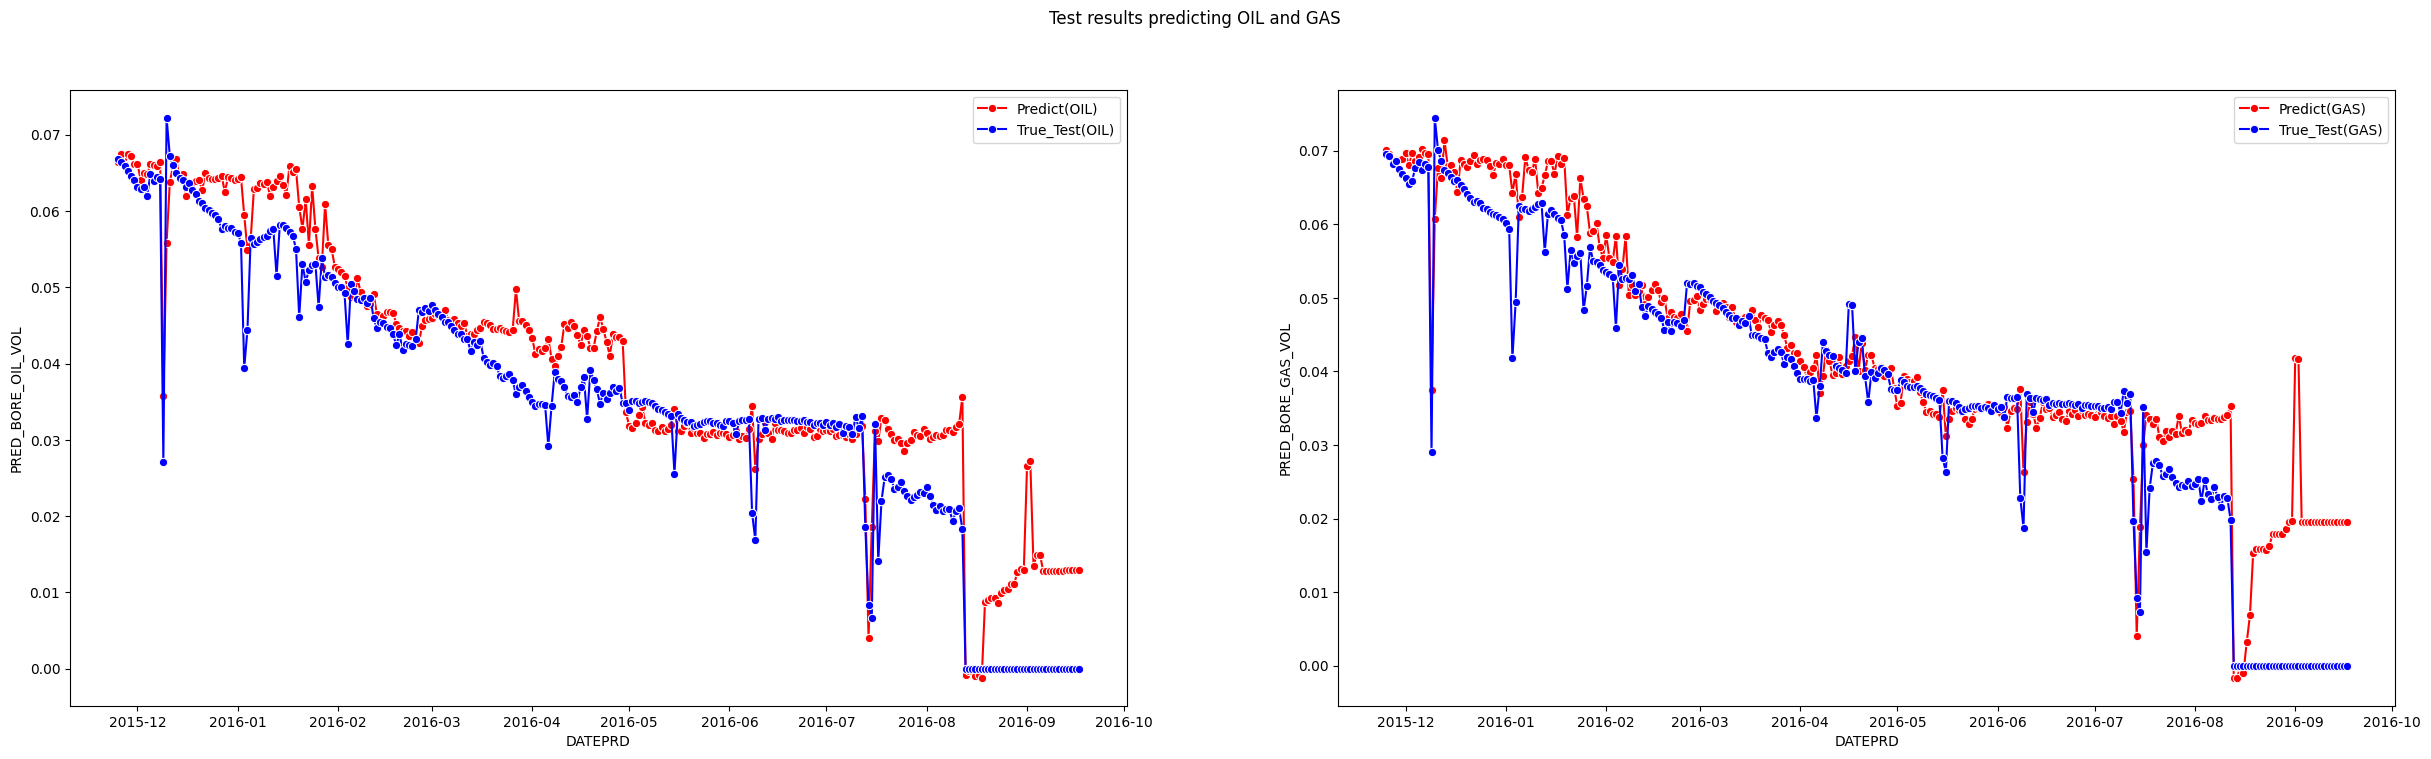
\includegraphics[width=1.0\textwidth]{images/Teste_lag_20.png}
    \caption{Test 20}
    \label{fig:Test_20}
\end{figure}